% DiffLaR Architecture Diagram - Standalone TikZ
\documentclass[tikz,border=10pt]{standalone}
\usepackage{tikz}
\usetikzlibrary{shapes,arrows,positioning,fit,backgrounds,calc}

\definecolor{llmblue}{RGB}{66,133,244}
\definecolor{diffgreen}{RGB}{52,168,83}
\definecolor{queryorange}{RGB}{251,188,5}
\definecolor{answerpurple}{RGB}{234,67,53}

\begin{document}
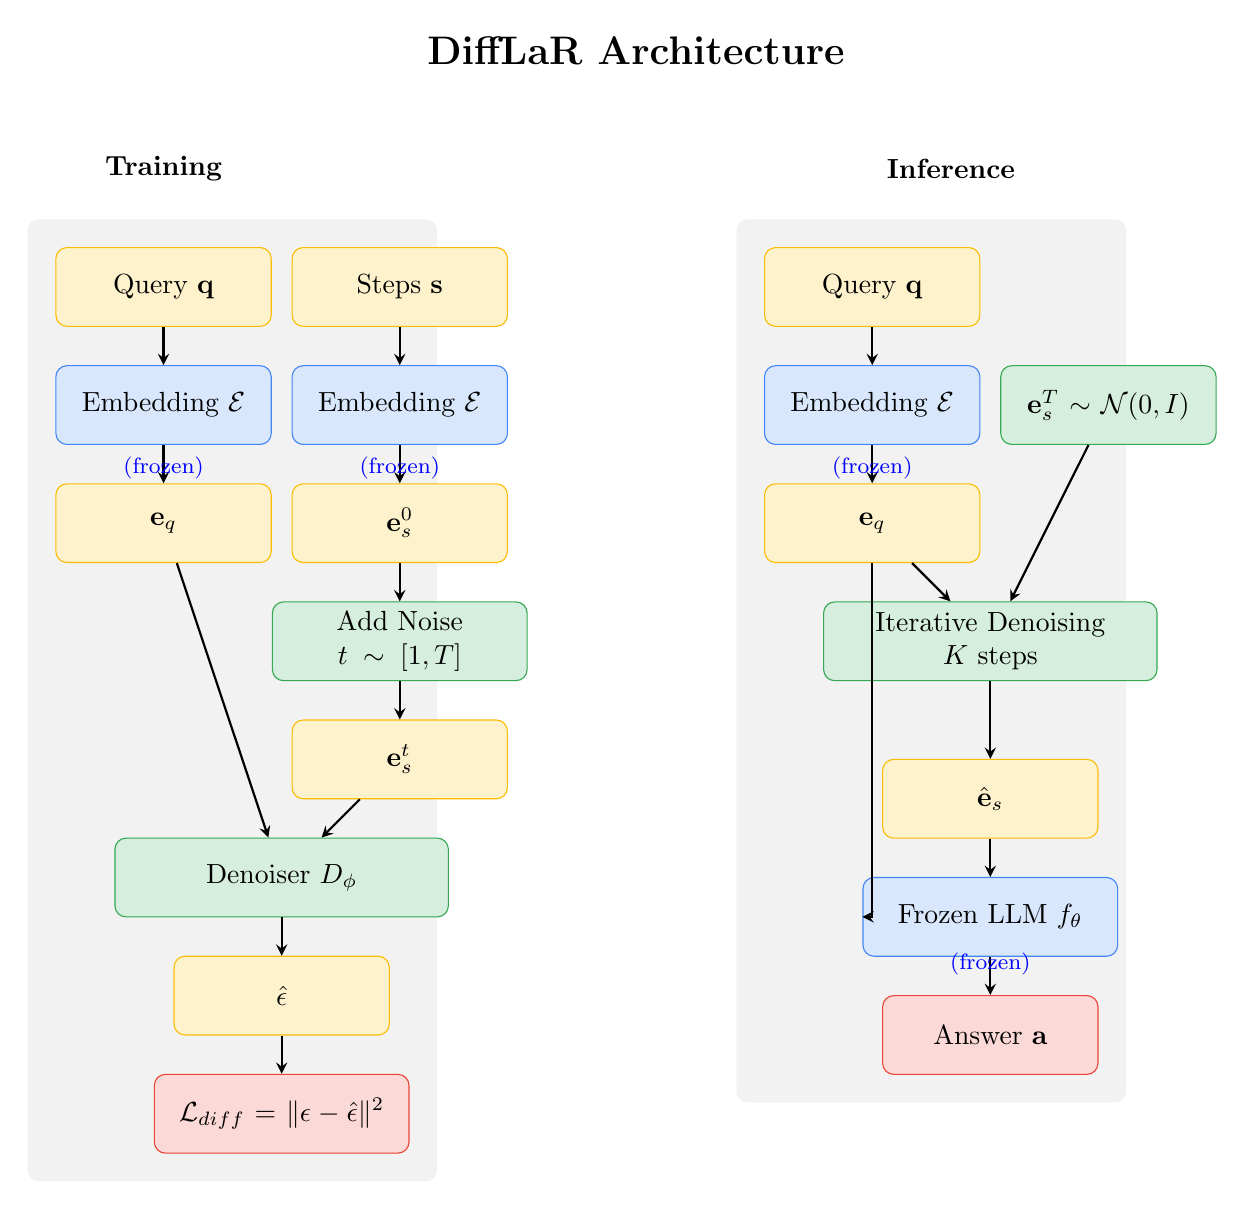
\begin{tikzpicture}[
    node distance=1.2cm,
    block/.style={rectangle, draw, fill=white, text width=2.5cm, text centered, minimum height=1cm, rounded corners},
    llmblock/.style={block, fill=llmblue!20, draw=llmblue},
    diffblock/.style={block, fill=diffgreen!20, draw=diffgreen},
    datablock/.style={block, fill=queryorange!20, draw=queryorange},
    outputblock/.style={block, fill=answerpurple!20, draw=answerpurple},
    arrow/.style={->, >=stealth, thick},
    dashedarrow/.style={->, >=stealth, thick, dashed}
]

% Title
\node[font=\Large\bfseries] (title) at (5,6) {DiffLaR Architecture};

% Left side - Training
\node[font=\bfseries] at (-1,4.5) {Training};

% Query path
\node[datablock] (query) at (-1,3) {Query $\mathbf{q}$};
\node[llmblock] (embed1) at (-1,1.5) {Embedding $\mathcal{E}$};
\node[datablock] (qembed) at (-1,0) {$\mathbf{e}_q$};

% Steps path
\node[datablock] (steps) at (2,3) {Steps $\mathbf{s}$};
\node[llmblock] (embed2) at (2,1.5) {Embedding $\mathcal{E}$};
\node[datablock] (sembed) at (2,0) {$\mathbf{e}_s^0$};

% Diffusion training
\node[diffblock, text width=3cm] (noise) at (2,-1.5) {Add Noise $t \sim [1,T]$};
\node[datablock] (noisy) at (2,-3) {$\mathbf{e}_s^t$};
\node[diffblock, text width=4cm] (denoiser) at (0.5,-4.5) {Denoiser $D_\phi$};
\node[datablock] (pred) at (0.5,-6) {$\hat{\epsilon}$};

% Loss
\node[outputblock, text width=3cm] (loss) at (0.5,-7.5) {$\mathcal{L}_{diff} = \|\epsilon - \hat{\epsilon}\|^2$};

% Arrows - Training
\draw[arrow] (query) -- (embed1);
\draw[arrow] (embed1) -- (qembed);
\draw[arrow] (steps) -- (embed2);
\draw[arrow] (embed2) -- (sembed);
\draw[arrow] (sembed) -- (noise);
\draw[arrow] (noise) -- (noisy);
\draw[arrow] (noisy) -- (denoiser);
\draw[arrow] (qembed) -- (denoiser);
\draw[arrow] (denoiser) -- (pred);
\draw[arrow] (pred) -- (loss);

% Right side - Inference
\node[font=\bfseries] at (9,4.5) {Inference};

% Query path inference
\node[datablock] (query2) at (8,3) {Query $\mathbf{q}$};
\node[llmblock] (embed3) at (8,1.5) {Embedding $\mathcal{E}$};
\node[datablock] (qembed2) at (8,0) {$\mathbf{e}_q$};

% Noise sampling
\node[diffblock] (sample) at (11,1.5) {$\mathbf{e}_s^T \sim \mathcal{N}(0,I)$};
\node[diffblock, text width=4cm] (denoise) at (9.5,-1.5) {Iterative Denoising\\$K$ steps};
\node[datablock] (generated) at (9.5,-3.5) {$\hat{\mathbf{e}}_s$};

% LLM generation
\node[llmblock, text width=3cm] (llm) at (9.5,-5) {Frozen LLM $f_\theta$};
\node[outputblock] (answer) at (9.5,-6.5) {Answer $\mathbf{a}$};

% Arrows - Inference
\draw[arrow] (query2) -- (embed3);
\draw[arrow] (embed3) -- (qembed2);
\draw[arrow] (sample) -- (denoise);
\draw[arrow] (qembed2) -- (denoise);
\draw[arrow] (denoise) -- (generated);
\draw[arrow] (generated) -- (llm);
\draw[arrow] (qembed2) -- ++(0,-5) -- (llm);
\draw[arrow] (llm) -- (answer);

% Background boxes
\begin{scope}[on background layer]
    \node[fit=(query)(loss), fill=gray!10, rounded corners, inner sep=10pt] {};
    \node[fit=(query2)(answer), fill=gray!10, rounded corners, inner sep=10pt] {};
\end{scope}

% Frozen indicator
\node[font=\footnotesize, text=blue] at (-1,0.7) {(frozen)};
\node[font=\footnotesize, text=blue] at (2,0.7) {(frozen)};
\node[font=\footnotesize, text=blue] at (8,0.7) {(frozen)};
\node[font=\footnotesize, text=blue] at (9.5,-5.6) {(frozen)};

\end{tikzpicture}
\end{document}
